
                \documentclass[8pt]{beamer} 
                \usetheme{CambridgeUS} 
                \usepackage{textpos} 
                \usepackage[latin1]{inputenc} 
                \usepackage{amsmath} 
                \usepackage{mathtools} 
                \usepackage{color} 
                \usepackage{mathabx} 
                \usepackage{graphicx} 
                \usepackage{tikz} 
                \usepackage{esvect} 
                \usetikzlibrary{arrows,shapes} 
                \usecolortheme{beaver} 
                \usepackage{graphicx} 
                \usepackage{changepage} 
                \setbeamertemplate{navigation symbols}{} 
                \setbeamertemplate{navigation symbols}{} 
            
        \title{GEANT4 Simulation Report}
        \author{Riccardo Nicolaidis \footnote{riccardo.nicolaidis@unitn.it}}
        \date{\today}
        
        \begin{document}
        
            \begin{frame}
                \titlepage
            \end{frame}
            
            \begin{frame}
                \frametitle{PID}
            
        \begin{figure}[h]
            \centering
            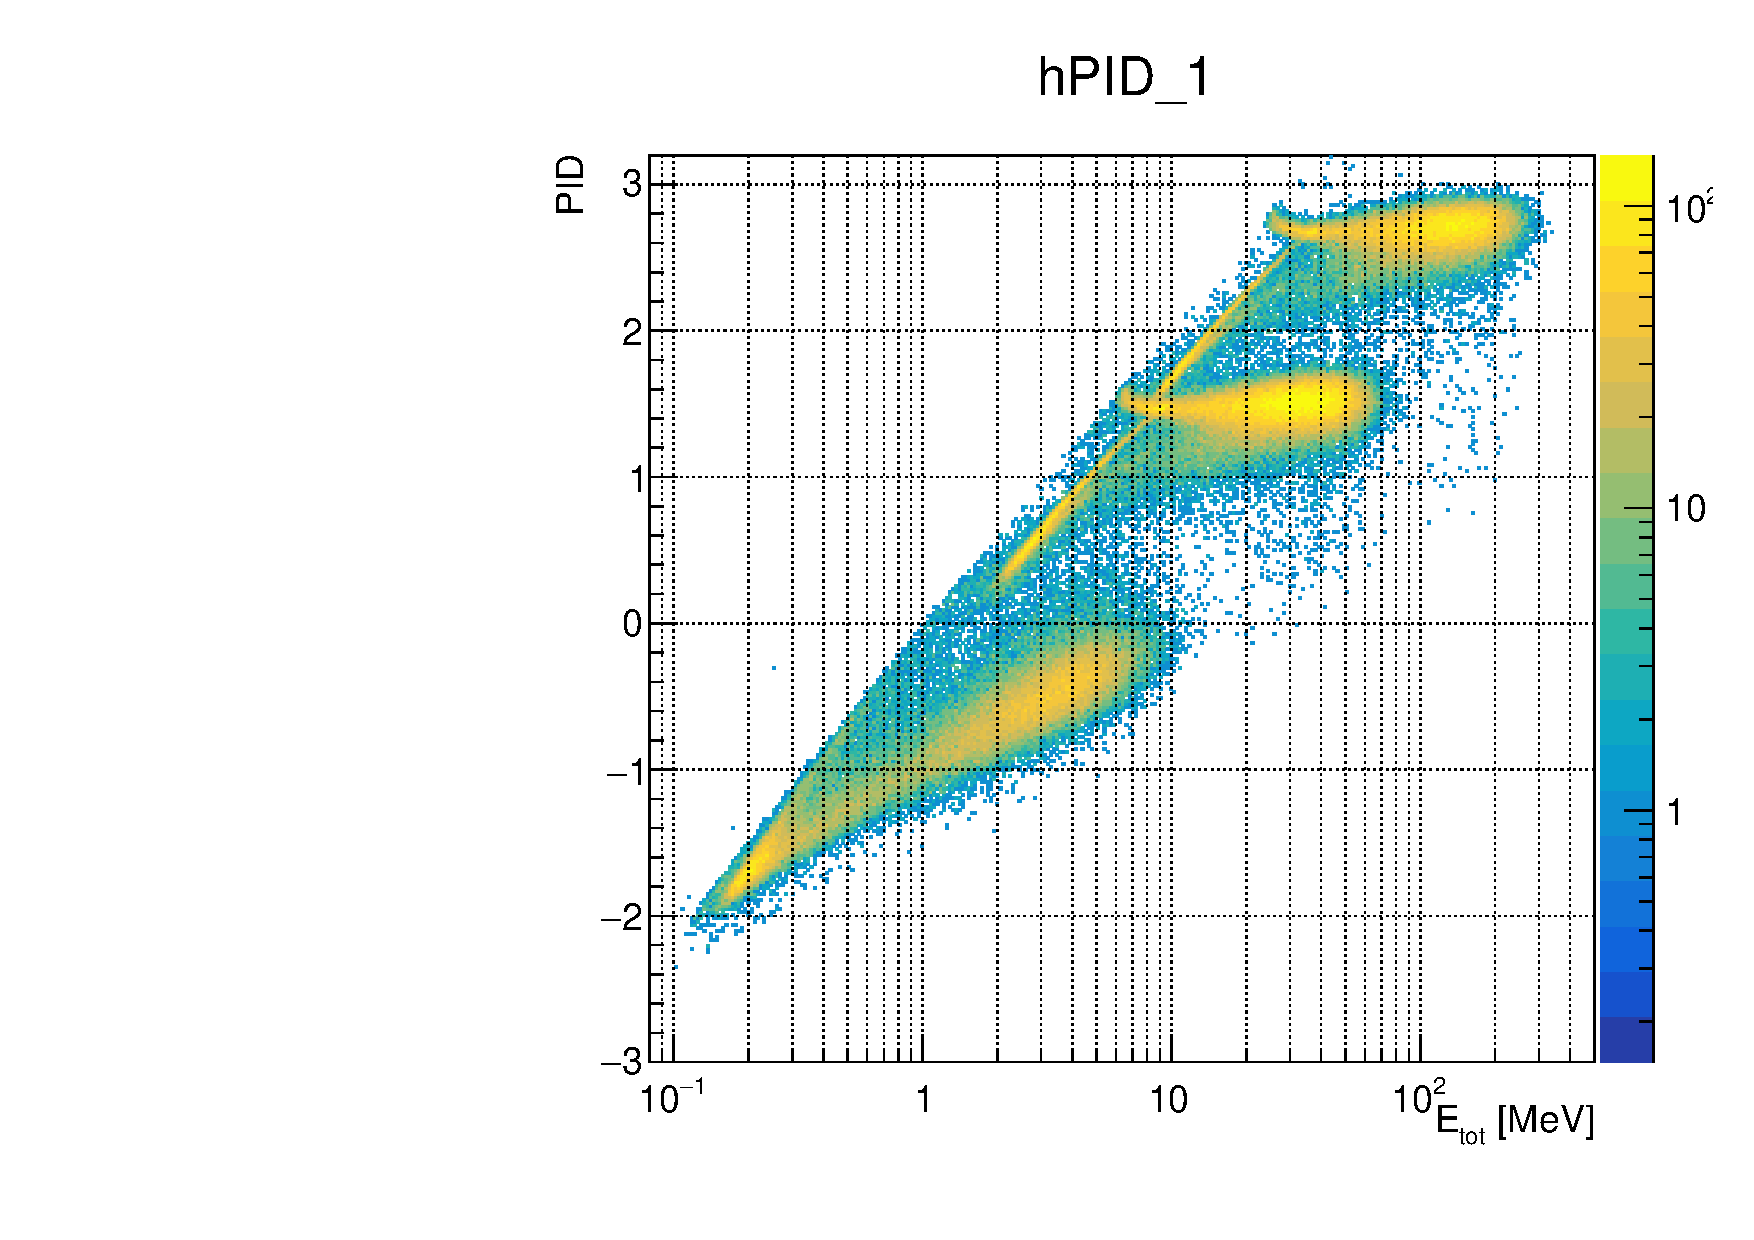
\includegraphics[width=0.5\textwidth]{/data1/home/rnicolai/LEM\_GDML\_upgrade/Output\_Geant4Simulation\_20230814/Analysis\_output/GDML\_file\_2/PID\_plots/gPID.pdf}
            \caption{PID, No Gaussian Smearing, Total Energy is the Energy reconstructed.}
        \end{figure}
        
            \end{frame}
            
            \begin{frame}
                \frametitle{PID No Calorimeter}
            
        \begin{figure}[h]
            \centering
            \includegraphics[width=0.5\textwidth]{/data1/home/rnicolai/LEM\_GDML\_upgrade/Output\_Geant4Simulation\_20230814/Analysis\_output/GDML\_file\_2/PID\_plots/gPID\_NoCalo.pdf}
            \caption{PID, No Gaussian Smearing, Total Energy is the Energy reconstructed, No Calorimeter.}
        \end{figure}
        
            \end{frame}
            
            \begin{frame}
                \frametitle{PID MC Energy}
            
        \begin{figure}[h]
            \centering
            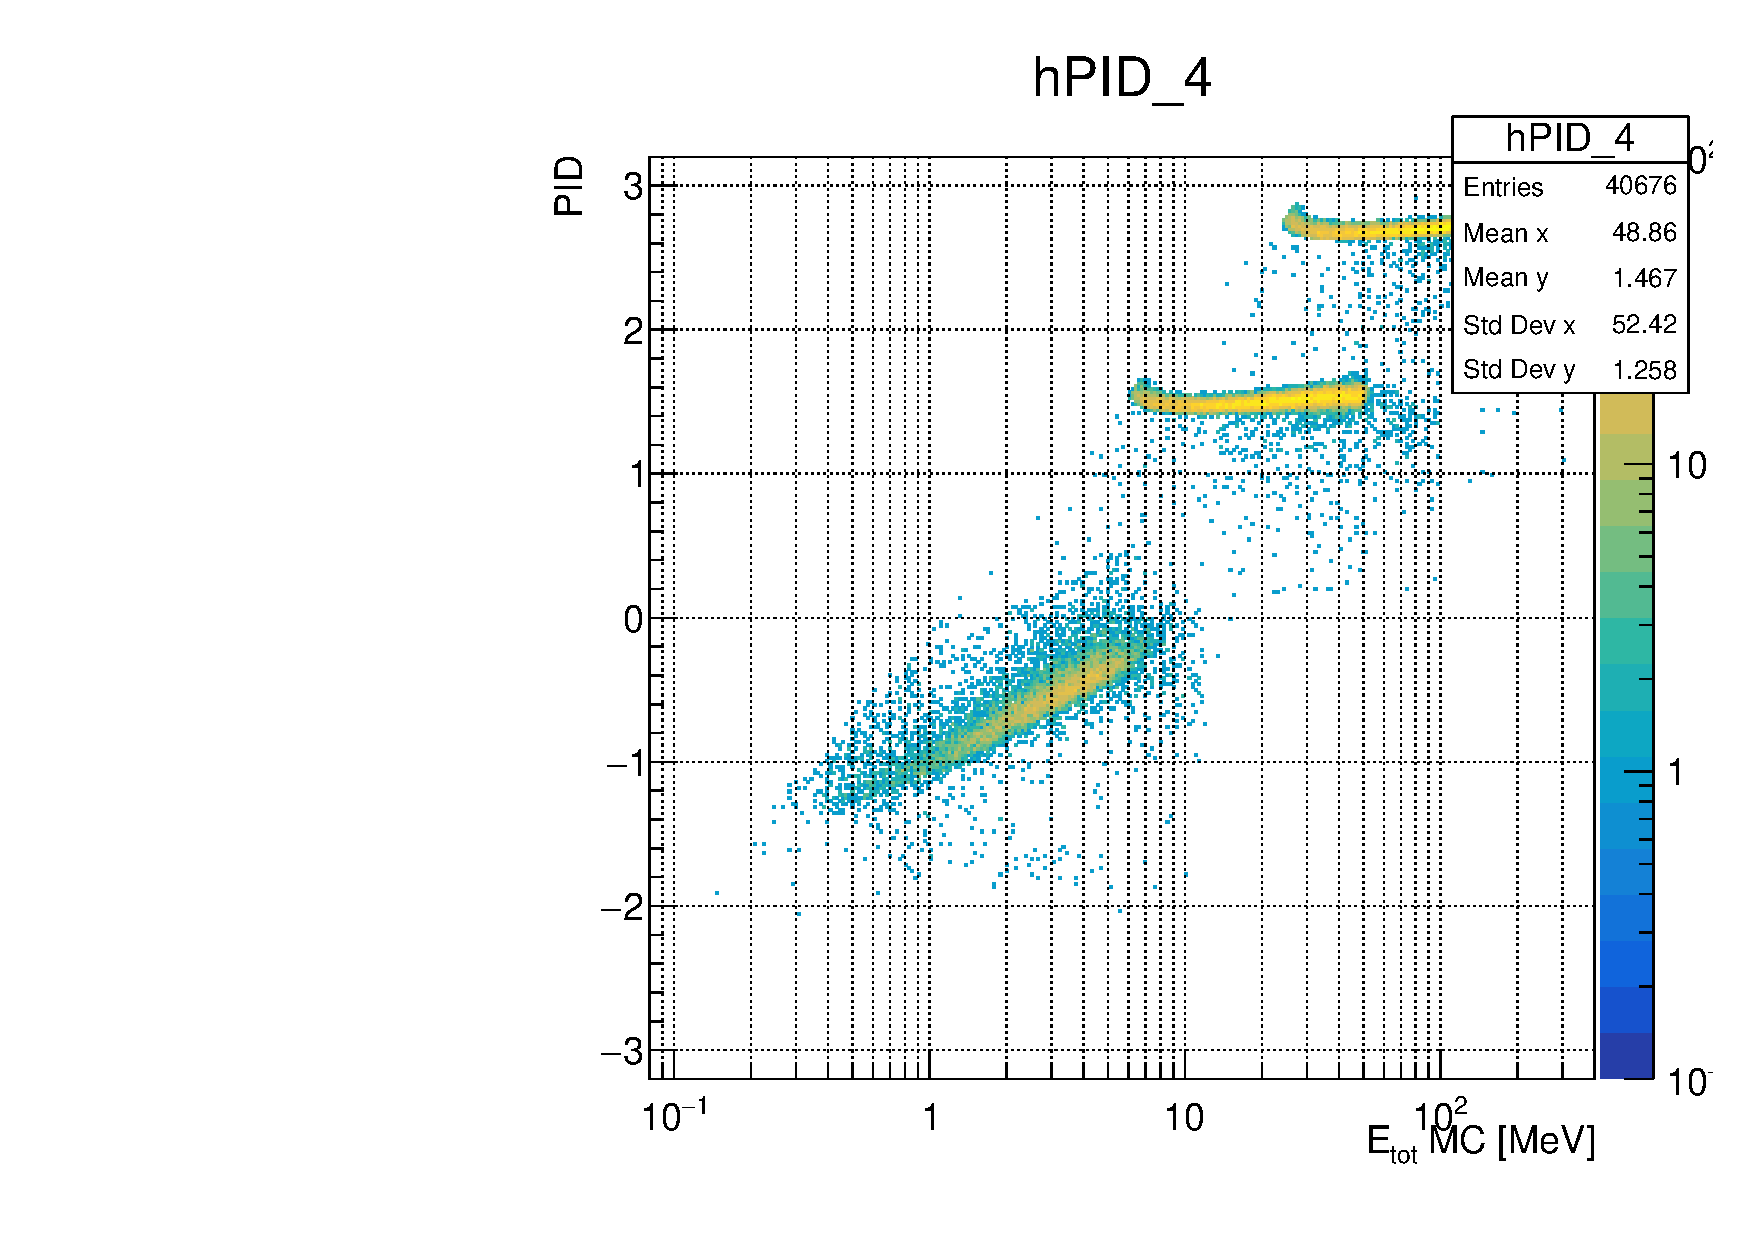
\includegraphics[width=0.5\textwidth]{/data1/home/rnicolai/LEM\_GDML\_upgrade/Output\_Geant4Simulation\_20230814/Analysis\_output/GDML\_file\_2/PID\_plots/PID2.pdf}
            \caption{PID, No Gaussian Smearing, Total Energy is the MC Energy.}
        \end{figure}
        
            \end{frame}
            
            \begin{frame}
                \frametitle{PID MC Energy No Calorimeter}
            
        \begin{figure}[h]
            \centering
            \includegraphics[width=0.5\textwidth]{/data1/home/rnicolai/LEM\_GDML\_upgrade/Output\_Geant4Simulation\_20230814/Analysis\_output/GDML\_file\_2/PID\_plots/gPID2\_NoCalo.pdf}
            \caption{PID, No Gaussian Smearing, Total Energy is the MC Energy, No Calorimeter.}
        \end{figure}
        
            \end{frame}
            
            \begin{frame}
                \frametitle{PID Gaussian Smearing}
            
        \begin{figure}[h]
            \centering
            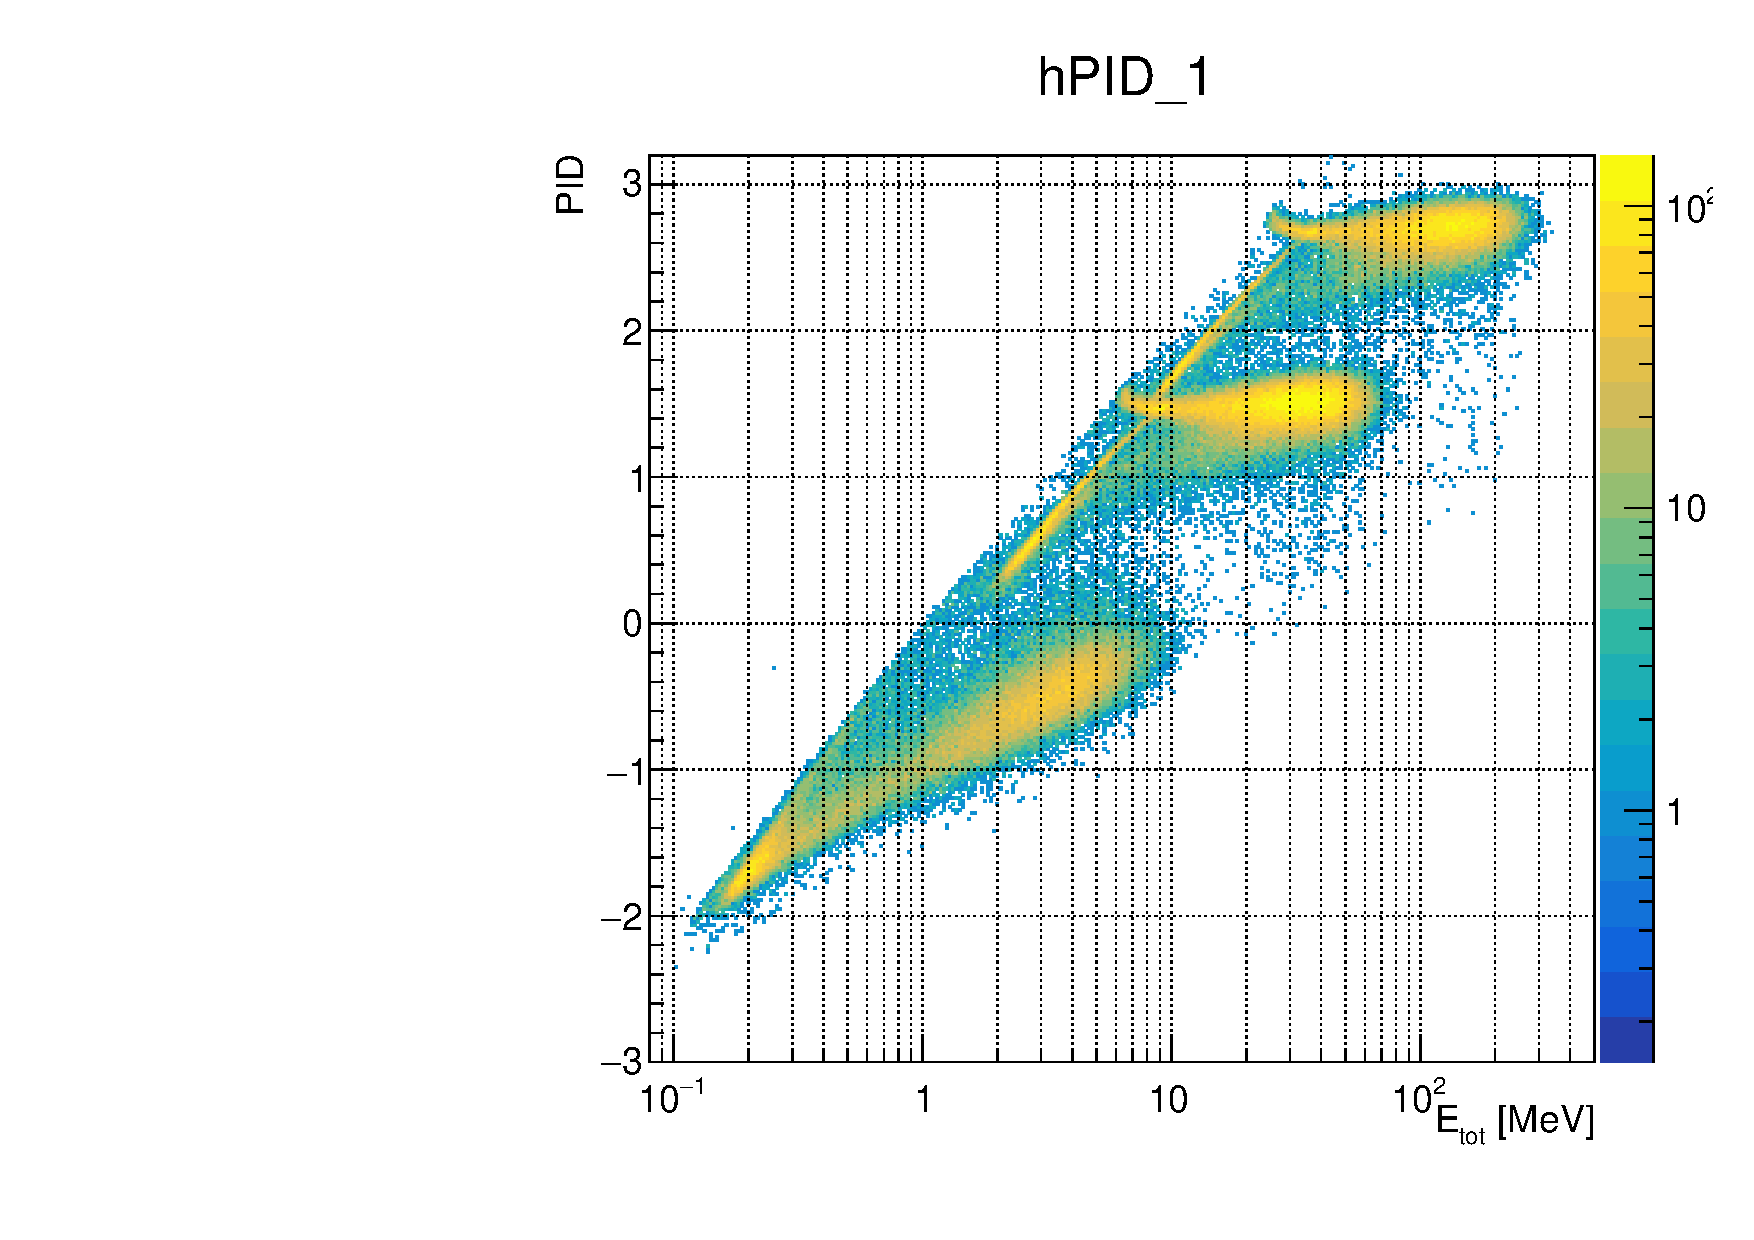
\includegraphics[width=0.5\textwidth]{/data1/home/rnicolai/LEM\_GDML\_upgrade/Output\_Geant4Simulation\_20230814/Analysis\_output/GDML\_file\_2/PID\_plots/gPID.pdf}
            \caption{PID, Gaussian Smearing, Total Energy is the Energy reconstructed.}
        \end{figure}
        
            \end{frame}
            
            \begin{frame}
                \frametitle{PID Gaussian Smearing No Calorimeter}
            
        \begin{figure}[h]
            \centering
            \includegraphics[width=0.5\textwidth]{/data1/home/rnicolai/LEM\_GDML\_upgrade/Output\_Geant4Simulation\_20230814/Analysis\_output/GDML\_file\_2/PID\_plots/gPID\_NoCalo.pdf}
            \caption{PID, Gaussian Smearing, Total Energy is the Energy reconstructed, No Calorimeter.}
        \end{figure}
        
            \end{frame}
            
            \begin{frame}
                \frametitle{PID MC Energy Gaussian Smearing}
            
        \begin{figure}[h]
            \centering
            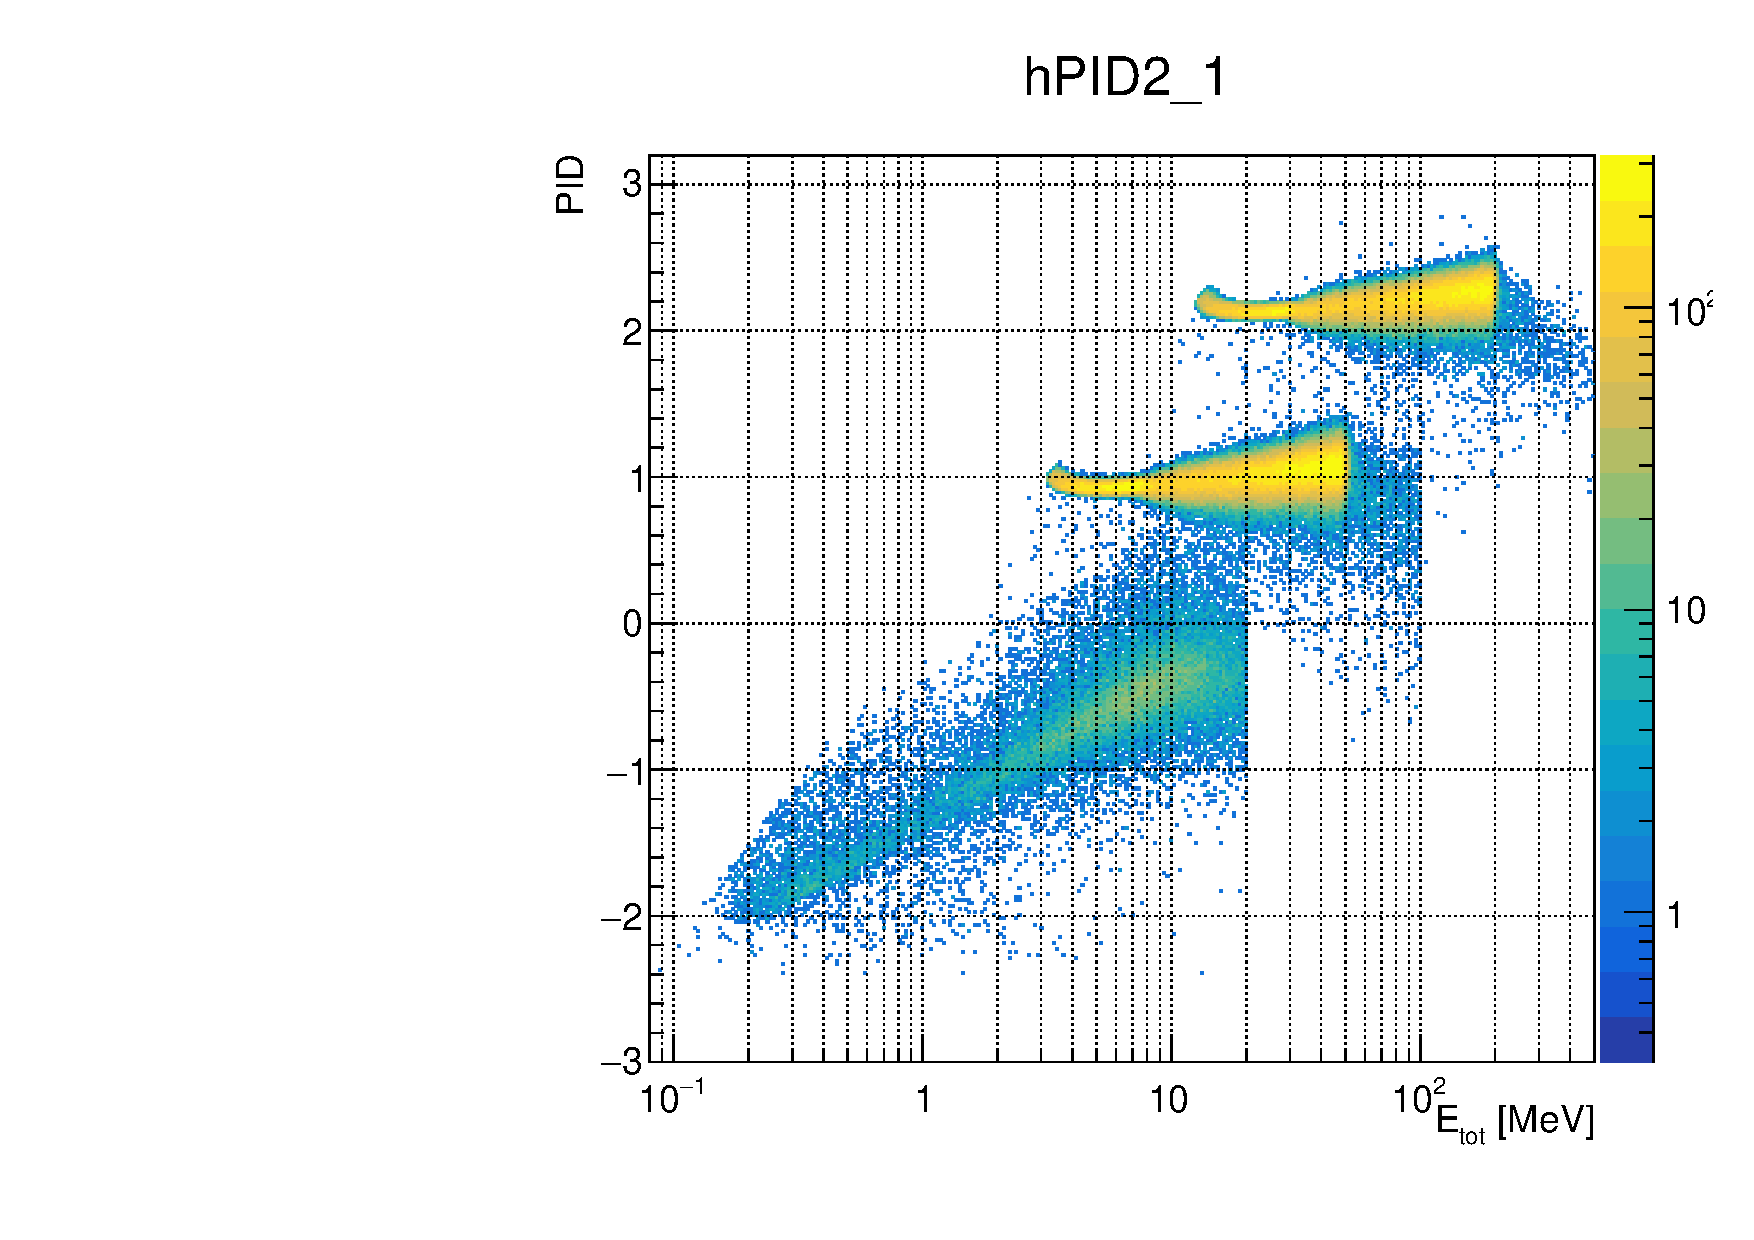
\includegraphics[width=0.5\textwidth]{/data1/home/rnicolai/LEM\_GDML\_upgrade/Output\_Geant4Simulation\_20230814/Analysis\_output/GDML\_file\_2/PID\_plots/gPID2.pdf}
            \caption{PID, Gaussian Smearing, Total Energy is the MC Energy.}
        \end{figure}
        
            \end{frame}
            
            \begin{frame}
                \frametitle{PID MC Energy Gaussian Smearing No Calorimeter}
            
        \begin{figure}[h]
            \centering
            \includegraphics[width=0.5\textwidth]{/data1/home/rnicolai/LEM\_GDML\_upgrade/Output\_Geant4Simulation\_20230814/Analysis\_output/GDML\_file\_2/PID\_plots/gPID2\_NoCalo.pdf}
            \caption{PID, Gaussian Smearing, Total Energy is the MC Energy, No Calorimeter.}
        \end{figure}
        
            \end{frame}
            
            \begin{frame}
                \frametitle{PID graphs}
            
        \begin{figure}[h]
            \centering
            \includegraphics[width=0.5\textwidth]{/data1/home/rnicolai/LEM\_GDML\_upgrade/Output\_Geant4Simulation\_20230814/Analysis\_output/GDML\_file\_2/PID\_plots/graph\_PID\_center.pdf}
            \caption{PID, Gaussian Smearing, Total Energy is the Energy reconstructed, No Calorimeter.}
        \end{figure}
        
            \end{frame}
            
            \begin{frame}
                \frametitle{MC quantities for e-\_t0}
            
        \begin{figure}[h]
            \centering
            \includegraphics[width=0.8\textwidth]{/data1/home/rnicolai/LEM\_GDML\_upgrade/Output\_Geant4Simulation\_20230814/Analysis\_output/GDML\_file\_2/Montecarlo\_e-\_t0.pdf}
            \caption{MC quantities}
        \end{figure}
        
            \end{frame}
            
            \begin{frame}
                \frametitle{Energies distribution for e-}
            
        \begin{figure}[h]
            \centering
            \includegraphics[width=0.8\textwidth]{/data1/home/rnicolai/LEM\_GDML\_upgrade/Output\_Geant4Simulation\_20230814/Analysis\_output/GDML\_file\_2/Energies\_e-\_t0.pdf}
            \caption{Detected energies}
        \end{figure}
        
            \end{frame}
            
            \begin{frame}
                \frametitle{Angles distribution accepted for e-}
            
        \begin{figure}[h]
            \centering
            \includegraphics[width=0.8\textwidth]{/data1/home/rnicolai/LEM\_GDML\_upgrade/Output\_Geant4Simulation\_20230814/Analysis\_output/GDML\_file\_2/Angles\_e-\_t0.pdf}
            \caption{Angles distribution}
        \end{figure}
        
            \end{frame}
            
            \begin{frame}
                \frametitle{Angles distribution accepted for e-}
            
        \begin{figure}[h]
            \centering
            \includegraphics[width=0.8\textwidth]{/data1/home/rnicolai/LEM\_GDML\_upgrade/Output\_Geant4Simulation\_20230814/Analysis\_output/GDML\_file\_2/2DAngHistoFigure\_4\_e-\_t0\_e-\_t0.pdf}
            \caption{Angles distribution}
        \end{figure}
        
            \end{frame}
            
            \begin{frame}
                \frametitle{Angles distribution accepted for e-}
            
        \begin{figure}[h]
            \centering
            \includegraphics[width=0.8\textwidth]{/data1/home/rnicolai/LEM\_GDML\_upgrade/Output\_Geant4Simulation\_20230814/Analysis\_output/GDML\_file\_2/2DAngHistoFigure\_1\_e-\_t0\_e-\_t0.pdf}
            \caption{Angles distribution}
        \end{figure}
        
            \end{frame}
            
            \begin{frame}
                \frametitle{Angles distribution accepted for e-}
            
        \begin{figure}[h]
            \centering
            \includegraphics[width=0.8\textwidth]{/data1/home/rnicolai/LEM\_GDML\_upgrade/Output\_Geant4Simulation\_20230814/Analysis\_output/GDML\_file\_2/2DAngHistoFigure\_2\_e-\_t0\_e-\_t0.pdf}
            \caption{Angles distribution}
        \end{figure}
        
            \end{frame}
            
            \begin{frame}
                \frametitle{Angles distribution accepted for e-}
            
        \begin{figure}[h]
            \centering
            \includegraphics[width=0.8\textwidth]{/data1/home/rnicolai/LEM\_GDML\_upgrade/Output\_Geant4Simulation\_20230814/Analysis\_output/GDML\_file\_2/2DAngHistoFigure\_3\_e-\_t0\_e-\_t0.pdf}
            \caption{Angles distribution}
        \end{figure}
        
            \end{frame}
            
            \begin{frame}
                \frametitle{Angles distribution accepted for e-}
            
        \begin{figure}[h]
            \centering
            \includegraphics[width=0.8\textwidth]{/data1/home/rnicolai/LEM\_GDML\_upgrade/Output\_Geant4Simulation\_20230814/Analysis\_output/GDML\_file\_2/2DAngHistoFigure\_0\_e-\_t0\_e-\_t0.pdf}
            \caption{Angles distribution}
        \end{figure}
        
            \end{frame}
            
            \begin{frame}
                \frametitle{Generation Position distribution accepted for e-}
            
        \begin{figure}[h]
            \centering
            \includegraphics[width=0.8\textwidth]{/data1/home/rnicolai/LEM\_GDML\_upgrade/Output\_Geant4Simulation\_20230814/Analysis\_output/GDML\_file\_2/GenPosition\_3\_e-\_t0\_e-\_t0.pdf}
            \caption{Generation Position}
        \end{figure}
        
            \end{frame}
            
            \begin{frame}
                \frametitle{Generation Position distribution accepted for e-}
            
        \begin{figure}[h]
            \centering
            \includegraphics[width=0.8\textwidth]{/data1/home/rnicolai/LEM\_GDML\_upgrade/Output\_Geant4Simulation\_20230814/Analysis\_output/GDML\_file\_2/GenPosition\_4\_e-\_t0\_e-\_t0.pdf}
            \caption{Generation Position}
        \end{figure}
        
            \end{frame}
            
            \begin{frame}
                \frametitle{Generation Position distribution accepted for e-}
            
        \begin{figure}[h]
            \centering
            \includegraphics[width=0.8\textwidth]{/data1/home/rnicolai/LEM\_GDML\_upgrade/Output\_Geant4Simulation\_20230814/Analysis\_output/GDML\_file\_2/GenPosition\_1\_e-\_t0\_e-\_t0.pdf}
            \caption{Generation Position}
        \end{figure}
        
            \end{frame}
            
            \begin{frame}
                \frametitle{Generation Position distribution accepted for e-}
            
        \begin{figure}[h]
            \centering
            \includegraphics[width=0.8\textwidth]{/data1/home/rnicolai/LEM\_GDML\_upgrade/Output\_Geant4Simulation\_20230814/Analysis\_output/GDML\_file\_2/GenPosition\_2\_e-\_t0\_e-\_t0.pdf}
            \caption{Generation Position}
        \end{figure}
        
            \end{frame}
            
            \begin{frame}
                \frametitle{Generation Position distribution accepted for e-}
            
        \begin{figure}[h]
            \centering
            \includegraphics[width=0.8\textwidth]{/data1/home/rnicolai/LEM\_GDML\_upgrade/Output\_Geant4Simulation\_20230814/Analysis\_output/GDML\_file\_2/GenPosition\_0\_e-\_t0\_e-\_t0.pdf}
            \caption{Generation Position}
        \end{figure}
        
            \end{frame}
            
            \begin{frame}
                \frametitle{Geometric factors for e-}
            
            \end{frame}
            
            \begin{frame}
                \frametitle{Geometric factors for e-}
            
            \end{frame}
            
            \begin{frame}
                \frametitle{MC quantities for proton\_t0}
            
        \begin{figure}[h]
            \centering
            \includegraphics[width=0.8\textwidth]{/data1/home/rnicolai/LEM\_GDML\_upgrade/Output\_Geant4Simulation\_20230814/Analysis\_output/GDML\_file\_2/Montecarlo\_proton\_t0.pdf}
            \caption{MC quantities}
        \end{figure}
        
            \end{frame}
            
            \begin{frame}
                \frametitle{Energies distribution for proton}
            
        \begin{figure}[h]
            \centering
            \includegraphics[width=0.8\textwidth]{/data1/home/rnicolai/LEM\_GDML\_upgrade/Output\_Geant4Simulation\_20230814/Analysis\_output/GDML\_file\_2/Energies\_proton\_t0.pdf}
            \caption{Detected energies}
        \end{figure}
        
            \end{frame}
            
            \begin{frame}
                \frametitle{Angles distribution accepted for proton}
            
        \begin{figure}[h]
            \centering
            \includegraphics[width=0.8\textwidth]{/data1/home/rnicolai/LEM\_GDML\_upgrade/Output\_Geant4Simulation\_20230814/Analysis\_output/GDML\_file\_2/Angles\_proton\_t0.pdf}
            \caption{Angles distribution}
        \end{figure}
        
            \end{frame}
            
            \begin{frame}
                \frametitle{Angles distribution accepted for proton}
            
        \begin{figure}[h]
            \centering
            \includegraphics[width=0.8\textwidth]{/data1/home/rnicolai/LEM\_GDML\_upgrade/Output\_Geant4Simulation\_20230814/Analysis\_output/GDML\_file\_2/2DAngHistoFigure\_2\_proton\_t0\_proton\_t0.pdf}
            \caption{Angles distribution}
        \end{figure}
        
            \end{frame}
            
            \begin{frame}
                \frametitle{Angles distribution accepted for proton}
            
        \begin{figure}[h]
            \centering
            \includegraphics[width=0.8\textwidth]{/data1/home/rnicolai/LEM\_GDML\_upgrade/Output\_Geant4Simulation\_20230814/Analysis\_output/GDML\_file\_2/2DAngHistoFigure\_1\_proton\_t0\_proton\_t0.pdf}
            \caption{Angles distribution}
        \end{figure}
        
            \end{frame}
            
            \begin{frame}
                \frametitle{Angles distribution accepted for proton}
            
        \begin{figure}[h]
            \centering
            \includegraphics[width=0.8\textwidth]{/data1/home/rnicolai/LEM\_GDML\_upgrade/Output\_Geant4Simulation\_20230814/Analysis\_output/GDML\_file\_2/2DAngHistoFigure\_4\_proton\_t0\_proton\_t0.pdf}
            \caption{Angles distribution}
        \end{figure}
        
            \end{frame}
            
            \begin{frame}
                \frametitle{Angles distribution accepted for proton}
            
        \begin{figure}[h]
            \centering
            \includegraphics[width=0.8\textwidth]{/data1/home/rnicolai/LEM\_GDML\_upgrade/Output\_Geant4Simulation\_20230814/Analysis\_output/GDML\_file\_2/2DAngHistoFigure\_3\_proton\_t0\_proton\_t0.pdf}
            \caption{Angles distribution}
        \end{figure}
        
            \end{frame}
            
            \begin{frame}
                \frametitle{Angles distribution accepted for proton}
            
        \begin{figure}[h]
            \centering
            \includegraphics[width=0.8\textwidth]{/data1/home/rnicolai/LEM\_GDML\_upgrade/Output\_Geant4Simulation\_20230814/Analysis\_output/GDML\_file\_2/2DAngHistoFigure\_0\_proton\_t0\_proton\_t0.pdf}
            \caption{Angles distribution}
        \end{figure}
        
            \end{frame}
            
            \begin{frame}
                \frametitle{Generation Position distribution accepted for proton}
            
        \begin{figure}[h]
            \centering
            \includegraphics[width=0.8\textwidth]{/data1/home/rnicolai/LEM\_GDML\_upgrade/Output\_Geant4Simulation\_20230814/Analysis\_output/GDML\_file\_2/GenPosition\_0\_proton\_t0\_proton\_t0.pdf}
            \caption{Generation Position}
        \end{figure}
        
            \end{frame}
            
            \begin{frame}
                \frametitle{Generation Position distribution accepted for proton}
            
        \begin{figure}[h]
            \centering
            \includegraphics[width=0.8\textwidth]{/data1/home/rnicolai/LEM\_GDML\_upgrade/Output\_Geant4Simulation\_20230814/Analysis\_output/GDML\_file\_2/GenPosition\_2\_proton\_t0\_proton\_t0.pdf}
            \caption{Generation Position}
        \end{figure}
        
            \end{frame}
            
            \begin{frame}
                \frametitle{Generation Position distribution accepted for proton}
            
        \begin{figure}[h]
            \centering
            \includegraphics[width=0.8\textwidth]{/data1/home/rnicolai/LEM\_GDML\_upgrade/Output\_Geant4Simulation\_20230814/Analysis\_output/GDML\_file\_2/GenPosition\_3\_proton\_t0\_proton\_t0.pdf}
            \caption{Generation Position}
        \end{figure}
        
            \end{frame}
            
            \begin{frame}
                \frametitle{Generation Position distribution accepted for proton}
            
        \begin{figure}[h]
            \centering
            \includegraphics[width=0.8\textwidth]{/data1/home/rnicolai/LEM\_GDML\_upgrade/Output\_Geant4Simulation\_20230814/Analysis\_output/GDML\_file\_2/GenPosition\_1\_proton\_t0\_proton\_t0.pdf}
            \caption{Generation Position}
        \end{figure}
        
            \end{frame}
            
            \begin{frame}
                \frametitle{Generation Position distribution accepted for proton}
            
        \begin{figure}[h]
            \centering
            \includegraphics[width=0.8\textwidth]{/data1/home/rnicolai/LEM\_GDML\_upgrade/Output\_Geant4Simulation\_20230814/Analysis\_output/GDML\_file\_2/GenPosition\_4\_proton\_t0\_proton\_t0.pdf}
            \caption{Generation Position}
        \end{figure}
        
            \end{frame}
            
            \begin{frame}
                \frametitle{Geometric factors for proton}
            
            \end{frame}
            
            \begin{frame}
                \frametitle{Geometric factors for proton}
            
            \end{frame}
            
            \begin{frame}
                \frametitle{MC quantities for alpha\_t0}
            
        \begin{figure}[h]
            \centering
            \includegraphics[width=0.8\textwidth]{/data1/home/rnicolai/LEM\_GDML\_upgrade/Output\_Geant4Simulation\_20230814/Analysis\_output/GDML\_file\_2/Montecarlo\_alpha\_t0.pdf}
            \caption{MC quantities}
        \end{figure}
        
            \end{frame}
            
            \begin{frame}
                \frametitle{Energies distribution for alpha}
            
        \begin{figure}[h]
            \centering
            \includegraphics[width=0.8\textwidth]{/data1/home/rnicolai/LEM\_GDML\_upgrade/Output\_Geant4Simulation\_20230814/Analysis\_output/GDML\_file\_2/Energies\_alpha\_t0.pdf}
            \caption{Detected energies}
        \end{figure}
        
            \end{frame}
            
            \begin{frame}
                \frametitle{Angles distribution accepted for alpha}
            
        \begin{figure}[h]
            \centering
            \includegraphics[width=0.8\textwidth]{/data1/home/rnicolai/LEM\_GDML\_upgrade/Output\_Geant4Simulation\_20230814/Analysis\_output/GDML\_file\_2/Angles\_alpha\_t0.pdf}
            \caption{Angles distribution}
        \end{figure}
        
            \end{frame}
            
            \begin{frame}
                \frametitle{Angles distribution accepted for alpha}
            
        \begin{figure}[h]
            \centering
            \includegraphics[width=0.8\textwidth]{/data1/home/rnicolai/LEM\_GDML\_upgrade/Output\_Geant4Simulation\_20230814/Analysis\_output/GDML\_file\_2/2DAngHistoFigure\_2\_alpha\_t0\_alpha\_t0.pdf}
            \caption{Angles distribution}
        \end{figure}
        
            \end{frame}
            
            \begin{frame}
                \frametitle{Angles distribution accepted for alpha}
            
        \begin{figure}[h]
            \centering
            \includegraphics[width=0.8\textwidth]{/data1/home/rnicolai/LEM\_GDML\_upgrade/Output\_Geant4Simulation\_20230814/Analysis\_output/GDML\_file\_2/2DAngHistoFigure\_4\_alpha\_t0\_alpha\_t0.pdf}
            \caption{Angles distribution}
        \end{figure}
        
            \end{frame}
            
            \begin{frame}
                \frametitle{Angles distribution accepted for alpha}
            
        \begin{figure}[h]
            \centering
            \includegraphics[width=0.8\textwidth]{/data1/home/rnicolai/LEM\_GDML\_upgrade/Output\_Geant4Simulation\_20230814/Analysis\_output/GDML\_file\_2/2DAngHistoFigure\_0\_alpha\_t0\_alpha\_t0.pdf}
            \caption{Angles distribution}
        \end{figure}
        
            \end{frame}
            
            \begin{frame}
                \frametitle{Angles distribution accepted for alpha}
            
        \begin{figure}[h]
            \centering
            \includegraphics[width=0.8\textwidth]{/data1/home/rnicolai/LEM\_GDML\_upgrade/Output\_Geant4Simulation\_20230814/Analysis\_output/GDML\_file\_2/2DAngHistoFigure\_1\_alpha\_t0\_alpha\_t0.pdf}
            \caption{Angles distribution}
        \end{figure}
        
            \end{frame}
            
            \begin{frame}
                \frametitle{Angles distribution accepted for alpha}
            
        \begin{figure}[h]
            \centering
            \includegraphics[width=0.8\textwidth]{/data1/home/rnicolai/LEM\_GDML\_upgrade/Output\_Geant4Simulation\_20230814/Analysis\_output/GDML\_file\_2/2DAngHistoFigure\_3\_alpha\_t0\_alpha\_t0.pdf}
            \caption{Angles distribution}
        \end{figure}
        
            \end{frame}
            
            \begin{frame}
                \frametitle{Generation Position distribution accepted for alpha}
            
        \begin{figure}[h]
            \centering
            \includegraphics[width=0.8\textwidth]{/data1/home/rnicolai/LEM\_GDML\_upgrade/Output\_Geant4Simulation\_20230814/Analysis\_output/GDML\_file\_2/GenPosition\_2\_alpha\_t0\_alpha\_t0.pdf}
            \caption{Generation Position}
        \end{figure}
        
            \end{frame}
            
            \begin{frame}
                \frametitle{Generation Position distribution accepted for alpha}
            
        \begin{figure}[h]
            \centering
            \includegraphics[width=0.8\textwidth]{/data1/home/rnicolai/LEM\_GDML\_upgrade/Output\_Geant4Simulation\_20230814/Analysis\_output/GDML\_file\_2/GenPosition\_4\_alpha\_t0\_alpha\_t0.pdf}
            \caption{Generation Position}
        \end{figure}
        
            \end{frame}
            
            \begin{frame}
                \frametitle{Generation Position distribution accepted for alpha}
            
        \begin{figure}[h]
            \centering
            \includegraphics[width=0.8\textwidth]{/data1/home/rnicolai/LEM\_GDML\_upgrade/Output\_Geant4Simulation\_20230814/Analysis\_output/GDML\_file\_2/GenPosition\_3\_alpha\_t0\_alpha\_t0.pdf}
            \caption{Generation Position}
        \end{figure}
        
            \end{frame}
            
            \begin{frame}
                \frametitle{Generation Position distribution accepted for alpha}
            
        \begin{figure}[h]
            \centering
            \includegraphics[width=0.8\textwidth]{/data1/home/rnicolai/LEM\_GDML\_upgrade/Output\_Geant4Simulation\_20230814/Analysis\_output/GDML\_file\_2/GenPosition\_0\_alpha\_t0\_alpha\_t0.pdf}
            \caption{Generation Position}
        \end{figure}
        
            \end{frame}
            
            \begin{frame}
                \frametitle{Generation Position distribution accepted for alpha}
            
        \begin{figure}[h]
            \centering
            \includegraphics[width=0.8\textwidth]{/data1/home/rnicolai/LEM\_GDML\_upgrade/Output\_Geant4Simulation\_20230814/Analysis\_output/GDML\_file\_2/GenPosition\_1\_alpha\_t0\_alpha\_t0.pdf}
            \caption{Generation Position}
        \end{figure}
        
            \end{frame}
            
            \begin{frame}
                \frametitle{Geometric factors for alpha}
            
            \end{frame}
            
            \begin{frame}
                \frametitle{Geometric factors for alpha}
            
            \end{frame}
            
            \begin{frame}
                \frametitle{Geometric factors for all particles}
            
            \end{frame}
            
        \end{document}
        